\section{Zusammenfassung und Diskussion}

In Versuch 234 beschäftigen wir uns mit der Untersuchung der Spektren verschiedener Lichtquellen. Hier unterscheiden wir zwischen Temperaturstrahlern und Nichttemperaturstrahlern. Temperaturstrahler, wie beispielsweise eine Glühlampe, basieren auf dem Phänomen, dass jeder Körper, dessen Temperatur größer als $0\si{\kelvin}$ ist, elektromagnetische Strahlung abstrahlt, deren Intensitätsverteilung abhängig von der Wellenlänge dem Planck'schen Strahlungsgesetz folgt. Bei den Nichttemperaturstrahlern ist die Erzeugung von Licht entweder auf Anregung von Atomzuständen, zum Beispiel bei einer Natriumdampflampe, oder der Rekombination von Elektron-Loch-Paaren in Halbleitern, also LEDs, zurückzuführen.

Im ersten Versuchsteil untersuchten wir das Spektrum des wohl bekanntesten Temperaturstrahlers, der Sonne. Mit einem Gitterspektroskop nahmen wir das Spektrum des Tageslichts einmal direkt und einmal durch ein Fenster auf. Wir konnten beobachten, dass es sich um ein kontinuierliches Spektrum handelt, wie es von Temperaturstrahlern zu erwarten ist. 

\begin{figure}[H]
  \centering
  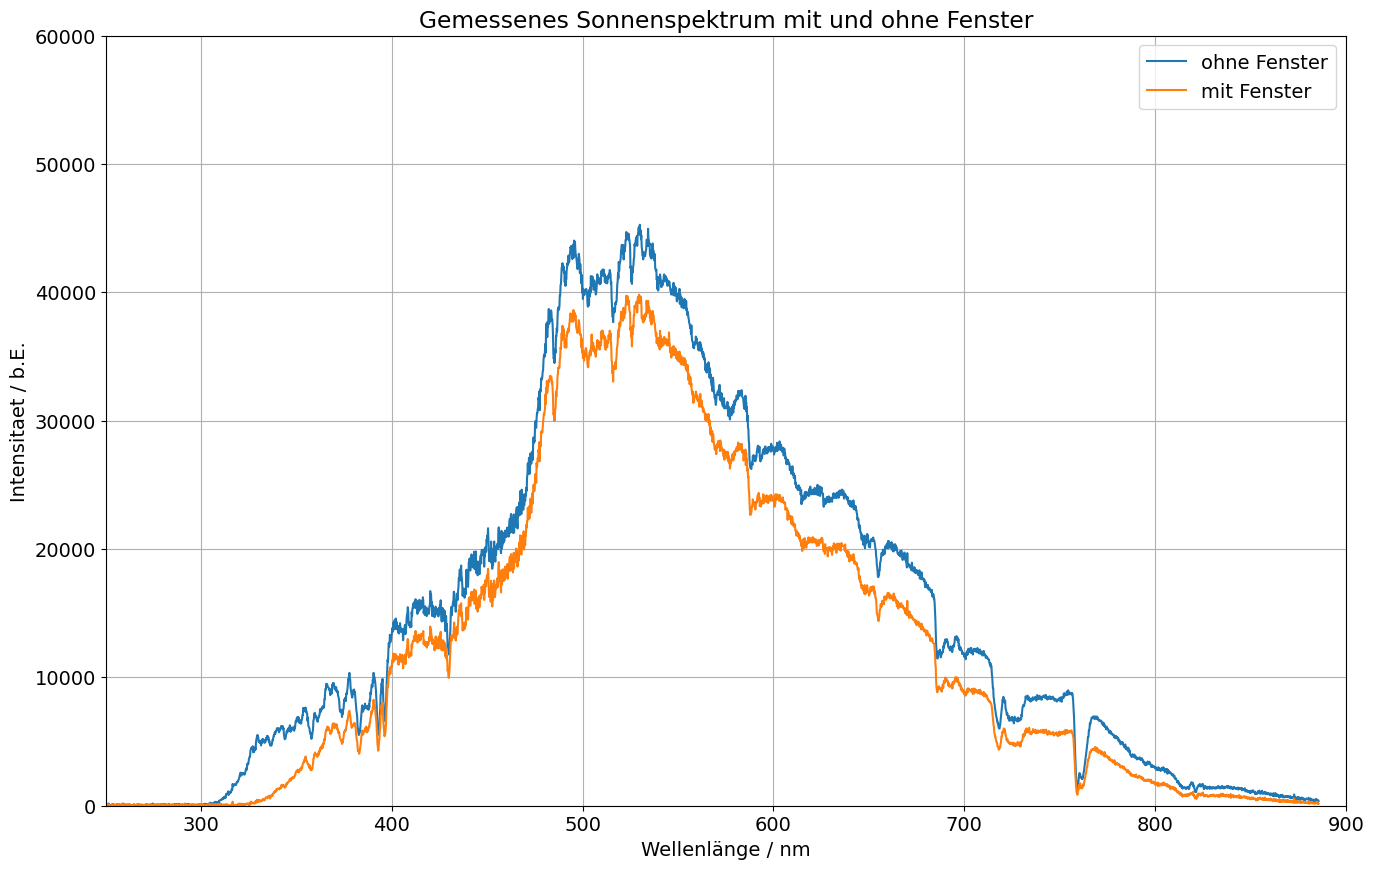
\includegraphics[width=.9\textwidth]{files/plots/himmel_m_o_g.png}
  \caption{Spektrum des Tageslichts mit und ohne Fenster.}
  \label{fig:himmel_m_o_g_zsmf}
\end{figure}


Im Vergleich des Spektrums durch das Fenster mit dem, das direkt aufgezeichnet wurde, konnten wir beobachten, dass durch die Scheibe über den gesamten Wellenlängenbereich hinweg die Intensität des Lichts durch die Absorption der Glasscheibe abgeschwächt wird. Bei genauerer Betrachtung der Absorption konnten wir sehen, dass diese im Bereich von Wellenlängen unter $400\si{\nano\meter}$, also im nicht-sichtbaren UV-Bereich, am höchsten und im Bereich des sichtbaren Lichts am niedrigsten ist.

Die vielen im Spektrum deutlich sichtbaren lokalen Minima sind durch die Absorption von Licht bestimmter Wellenlängen in den Atmosphärenschichten der Sonne und der Erde zu erklären. Diese Absorptionslinien, genannt \glqq{}Fraunhoferlinien\grqq{} sind speziellen Wellenlängen zugeordnet, welche wir mit den Positionen der Linien in unsren aufgezeichneten Spektrum verglichen. Die Werte sind, mit der jeweiligen Abweichung vom Literaturwert in \tabref{tab:frauenhofer_vergleich_zsmf} zusammengefasst. Als Fehler für die beobachteten Wellenlängen sind wir jeweils von $\pm 1\si{\nano\meter}$ ausgegangen.

\begin{table}[h]
  \centering
  \caption{Vergleich der erwarteten und gemessenen Wellenlängen der Frauenhoferlinien}
  \vspace*{0.5em}
  \begin{tabular}{c|c|c|c}
      \hline
      Linie & Literaturwert [nm] & Abgelesener Wert [nm] & Abweichung [$\sigma$] \\
      \hline
      K  & 393.4 & 393.0 & 0.4 \\
      H  & 396.8 & 396.1 & 0.7 \\
      G  & 430.8 & 429.8 & 1.0 \\
      F  & 486.1 & 485.2 & 0.91 \\
      b1 & 518.4 & 516.7 & 1.7 \\
      E  & 527.0 & 526.2 & 0.8 \\
      D3 & 587.6 & 588.4 & 0.8 \\
      D2 & 589.0 & 589.0 & 0.0 \\
      D1 & 589.6 & 589.7 & 0.11 \\
      C  & 656.3 & 655.0 & 1.3 \\
      B  & 686.7 & 686.7 & 0.0 \\
      A  & 759.4 & 759.4 & 0.0 \\
      \hline
  \end{tabular}
  \label{tab:frauenhofer_vergleich_zsmf}
\end{table}

Unter anderem also lokale Minima im Sonnenlichtspektrum zu beobachten sind die Linien der Balmerserie, welche auf Anregungen in Wasserstoffatom zurückzuführen sind. Die beobachteten Positionen der $H_{\alpha}-, H_{\beta}-, H_{\gamma}-, H_{\delta}-$Linien der Balmerserie verglichen wir ebenfalls mit den Literaturwerten, zusammengefasst in \tabref{}.

Insgesamt ist die Abweichung der beobachteten Absorptionslinien von den Literaturwerten sehr gering. Die dennoch sichtbaren Unterschieden sind vermutlich zu Großteilen auf das wolkige Wetter am Versuchstag, sowie Störungen und Reflexionen durch die umliegenden Gebäude zurückzuführen.

Im darauf folgenden Versuchsteil betrachteten wir qualitativ die Spektren verschiedener Lichtquellen. Hierunter untersuchten wir das Licht verschiedenfarbiger LEDs, eines Lasers und einer Energiesparlampe als Beispiele für Nichttemperaturstrahler, sowie das einer Glühlampe als ein klassisches Beispiel für einen Temperaturstrahler.